%!TEX root = ../template.tex
%%%%%%%%%%%%%%%%%%%%%%%%%%%%%%%%%%%%%%%%%%%%%%%%%%%%%%%%%%%%%%%%%%%
%% chapter1.tex
%% NOVA thesis document file
%%
%% Chapter with introduction
%%%%%%%%%%%%%%%%%%%%%%%%%%%%%%%%%%%%%%%%%%%%%%%%%%%%%%%%%%%%%%%%%%%

\typeout{NT FILE chapter1.tex}%

\chapter{Introduction}
\label{cha:introduction}

\prependtographicspath{{Chapters/Figures/Covers/phd/}{Chapters/Figures/Covers/msc/}}

% epigraph configuration
\epigraphfontsize{\small\itshape}
\setlength\epigraphwidth{12.5cm}
\setlength\epigraphrule{0pt}


\includegraphics[width=\linewidth]{NOVAthesisFiles/Images/novathesis-text}

\noindent This is the \novathesis\ \LaTeX\ template Version \novathesisversion\ from \novathesisdate.

\epigraph{
  This work is licensed under the \href{https://www.latex-project.org/lppl/lppl-1-3c/}{\LaTeX\ Project Public License v1.3c}.
  To view a copy of this license, visit the \href{https://www.latex-project.org/lppl/}{LaTeX project public license}.
}

\section{If You Use this Template…} 
\label{sub:if_you_use_this_template}

This first Chapter introduces the \gls{novathesis} template and how it is organized. In Chapter~\ref{cha:users_manual} you can find some specific instructions on how to use the \gls{novathesis} template.  Chapter~\ref{cha:a_short_latex_tutorial_with_examples} shows some examples and give some hints on how to write your text. Please read these next Chapters carefully.

\begin{quote}
  \rule{\linewidth}{2pt}
If you are going to spend zillions of hours writing your thesis/dissertation using this \gls{novathesis} template, be wise and spend a couple of hours learning how to use it properly and read this manual.  And then spend even a few more hours \href{https://github.com/joaomlourenco/novathesis/wiki#learning-latex}{learning some \LaTeX}.  I am sure the time you invest now will pay itself countless times before you submit your thesis/dissertation.
\hfill \raisebox{-1ex}{\itshape João Lourenço}\\[-1ex]
  \rule{\linewidth}{2pt}
\end{quote}

\subsection{Appeal}
\label{sub:appeal}

The \gls{novathesis} tempalte was born in~1996, and what you see now accumulates to many many hundreds (thousands?!) of working hours, unpaid and stollen from family and friends.  This work is available to the community under the \href{LaTeX project public license}{\LaTeX\ Project Public License v1.3c}, which means you are entitled to use it for free.  However, if you decide to use this template to write your thesis/dissertation, \textbf{be fair to the developers} and:
\begin{enumerate}
  \item Cite the \gls{novathesis} manual~\cite{novathesis-manual} in a place of your choice (e.g., in the \emph{Acknowledgments}) of your thesis/disseration with “\verb!\cite{novathesis-manual}!” .  If you cite it this way, the correct entry will be added automatically to your bibliography (no need to worry with the necessary BibTeX entry, as it will be added automatically);
  \item Go to the
\href{https://github.com/joaomlourenco/novathesis}{project web page in GitGub} and give the project a star (marked with a red ellipse at the top-right in Figure~\ref{fig:github}); and
  \item Make a donation by visiting the \gls{novathesis} project page and clicking in the button marked with a green ellipse at the top-center in Figure~\ref{fig:github}).  Alternatively, just click \href{https://www.paypal.com/donate/?hosted_button_id=8WA8FRVMB78W8}{\fcolorbox{DarkGreen}{gray!15}{\textbf{~HERE~}}} and your browser will be directed to the right page.
\end{enumerate}

\begin{figure}[htbp]
  \centering
    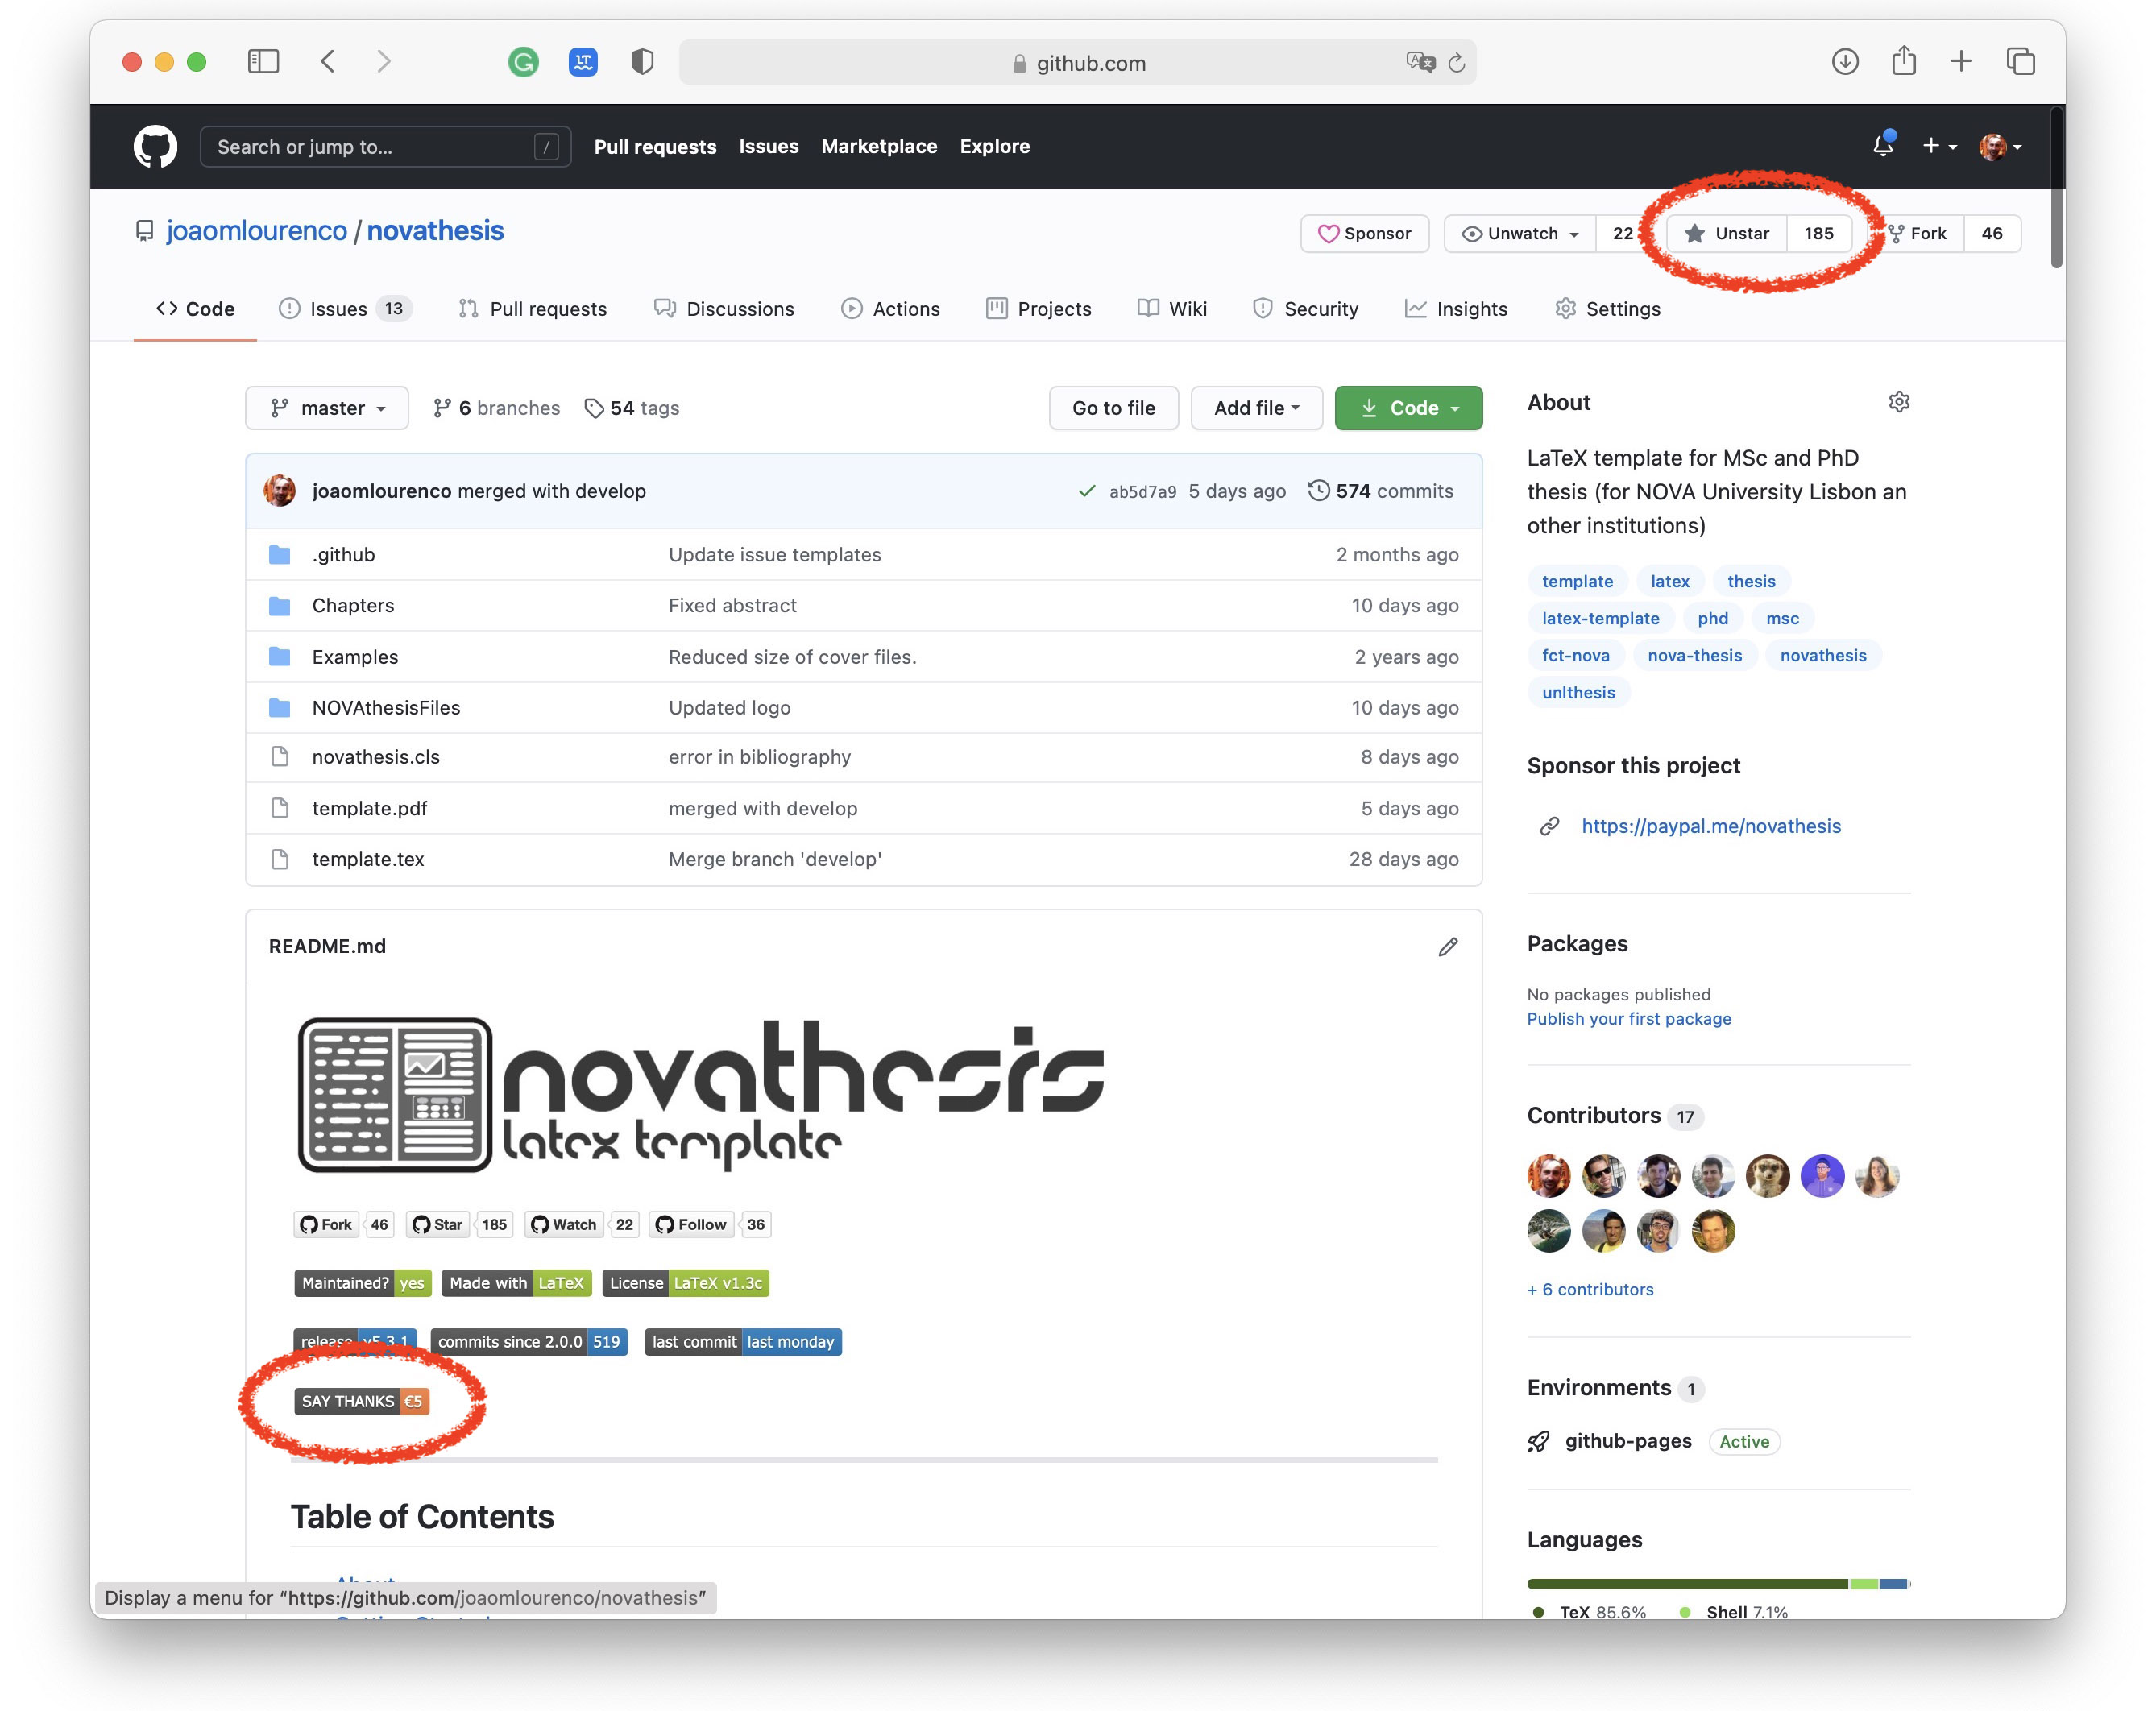
\includegraphics[width=0.8\textwidth]{github1}
  \caption{The \novathesis\ project web page in GitHub.}
  \label{fig:github}
\end{figure}


\section{The \emph{NOVAthesis} template}
\label{sec:a_bit_of_history}

\newcommand{\mysmallcoversize}{0.09\linewidth}
\renewcommand{\theadfont}{\large\bfseries}
\definecolor{Schlgray}{gray}{0.95}  
\newtoggle{ntRow}

\newcommand{\ntSchool}[4]{%
    % #1 = cover image
    % #2 = School name
    % #3 = School acronym
    % #3 = School URL
    \iftoggle{ntRow}{\rowcolor{GhostWhite}\global\togglefalse{ntRow}}{\global\toggletrue{ntRow}}
    \setlength{\fboxsep}{0pt}%
    \def\myspace{}%
    \makecell*[cc]{%
      \@for\listitem:=#1\do{%
        \myspace\fbox{\colorbox{White}{\includegraphics[width=\mysmallcoversize]{\listitem}}}\def\myspace{~}}%
    }
    & #2 \href{#4}{(#3)}\\%
}

\newenvironment{ntUniversity}[1]{
    \togglefalse{ntRow}
    \xltabular{\linewidth}{lX}%
    \toprule%
    \rowcolor{Gainsboro}%
    & \Gape[1.5ex]{\thead[l]{#1}}\\
    \midrule%
}{%
    \bottomrule
    \endxltabular%
}

The \gls{novathesis} template was initially directed to the PhD and MSc thesis/dissertations at the \gls{DI} of  \gls{FCT} of \gls{NOVA}, Portugal.  But the user base grew to other Departments of FCT-NOVA, then to other Schools and later to other Universities.  Currently more than 25 Schools are natively supported by the \gls{novathesis} teamplte.

\begin{ntUniversity}{NOVA University Lisbon}
    \ntSchool{cover-nova-fct-phd,cover-nova-fct-msc}%
                  {NOVA School of Science and Technology [PhD]}%
                  {FCT-NOVA}%
                  {https://www.fct.unl.pt}
    % \ntSchool{cover-nova-fct-msc}%
    %               {NOVA School of Science and Technology [MSc]}%
    %               {FCT-NOVA}%
    %               {https://www.fct.unl.pt}
    \ntSchool{cover-nova-fcsh-phd}%
                  {NOVA School of Social Sciences and Humanities}%
                  {FCSH-NOVA}%
                  {https://www.fcsh.unl.pt}
    \ntSchool{cover-nova-ims-phd}%
                  {NOVA Information Management School}%
                  {NOVA-IMS}%
                  {https://www.novaims.unl.pt}
    \ntSchool{cover-nova-ensp-phd}%
                  {National School of Public Heath}%
                  {ENSP-NOVA}%
                  {https://www.ensp.unl.pt}
\end{ntUniversity}

\begin{ntUniversity}{University of Lisbon}
    \ntSchool{cover-ulisboa-ist-phd}%
                  {Instituto Superior Técnico}%
                  {IST-UL}%
                  {https://tecnico.ulisboa.pt}
    \ntSchool{cover-ulisboa-fc-phd}%
                  {Faculdade de Ciências [PhD]}%
                  {FCUL}%
                  {https://ciencias.ulisboa}
    \ntSchool{cover-ulisboa-fc-msc}%
                  {Faculdade de Ciências [MSc]}%
                  {FCUL}%
                  {https://ciencias.ulisboa}
\end{ntUniversity}

\begin{ntUniversity}{University of Minho}
    \ntSchool{cover-uminho-ea-phd}%
                  {Escola de Arquitetura}%
                  {EA-UM}%
                  {https://www.arquitetura.uminho.pt}
    \ntSchool{cover-uminho-ec-phd}%
                  {Escola de Ciências}%
                  {EC-UM}%
                  {https://www.ecum.uminho.pt}
    \ntSchool{cover-uminho-ed-phd}%
                  {Escola de Direito}%
                  {ED-UM}%
                  {https://www.direito.uminho.pt}
    \ntSchool{cover-uminho-eeg-phd}%
                  {Escola de Economia e Gestão}%
                  {EEG-UM}%
                  {https://www.eeg.uminho.pt}
    \ntSchool{cover-uminho-ee-phd}%
                  {Escolha de Engenharia}%
                  {EE-UM}%
                  {https://www.eng.uminho.pt}
    \ntSchool{cover-uminho-em-phd}%
                  {Escola de Medicina}%
                  {EM-UM}%
                  {https://www.med.uminho.pt}
    \ntSchool{cover-uminho-ep-phd}%
                  {Escola de Psicologia}%
                  {EP-UM}%
                  {https://www.psi.uminho.pt}
    \ntSchool{cover-uminho-ese-phd}%
                  {Escola Superior de Enfermagem}%
                  {ESE-UM}%
                  {https://www.ese.uminho.pt}
    \ntSchool{cover-uminho-ics-phd}%
                  {Instituto de Ciências Sociais}%
                  {ICS-UM}%
                  {https://www.ilch.uminho.pt}
    \ntSchool{cover-uminho-ie-phd}%
                  {Instituto de Educação}%
                  {IE-UM}%
                  {https://www.ie.uminho.pt}
    \ntSchool{cover-uminho-ilch-phd}%
                  {Instituto de Letras e Ciências Humanas}%
                  {ILCH-UM}%
                  {https://www.ilch.uminho.pt}
    \ntSchool{cover-uminho-i3b-phd}%
                  {Instituto de Investigação em Biomateriais, Biodegradáveis e Biomiméticos}%
                  {I3B-UM}%
                  {https://i3bs.uminho.pt}
\end{ntUniversity}

\begin{ntUniversity}{ISCTE — Instituto Universitário de Lisboa}
    \ntSchool{cover-iscteiul-eta-phd}%
             {Escola de Tecnologias e Arquitectura}%
             {ETA-ISCTE-IUL}%
             {https://ciencia.iscte-iul.pt/schools/escola-tecnologias-arquitectura}%
\end{ntUniversity}

\begin{ntUniversity}{Instituto Politécnico de Lisboa}
    \ntSchool{cover-ipl-isel-msc}%
             {Instituto Superior de Engenharia de Lisboa}%
             {ISEL-IPL}%
             {https://www.isel.pt}%
\end{ntUniversity}

\begin{ntUniversity}{Instituto Politécnico de Setúbal}
    \ntSchool{cover-ips-ests-msc}%
             {Escola Superior de Tecnologia de Setúbal}%
             {ISEL-IPL}%
             {https://www.estbarreiro.ips}%
\end{ntUniversity}

\begin{ntUniversity}{Other Universities/Schools/Degrees}
    \ntSchool{cover-other-esep-phd}%
             {Escola Superior de Enfermagem do Porto}%
             {ESEP}%
             {https://www.esenf.pt/pt}%
    \ntSchool{cover-other-mscgt-msc}%
             {Masters Program in Geospatial Technologies}%
             {GT}%
             {https://mastergeotech.info}%
\end{ntUniversity}


\section{Getting Started}
\label{sec:getting_started}

The template provides an \emph{easy to use} setting for you to write your thesis/dissertation in \LaTeX:
\begin{itemize}
  \item  Select your school;
  \item Fill your thesis metadata (title, research field, etc) in the file “\texttt{template.tex}”;
  \item Create your thesis/dissertation contents using the files in folder “\texttt{Chapters}”; and
  \item Process using you favorite \LaTeX\ processor (pdf\LaTeX, \XeLaTeX\ or \LuaLaTeX).
\end{itemize}

\subsection{Using Overleaf}
\label{sub:using_overleaf}

\begin{wrapfigure}{r}{0.5\linewidth}
\vspace*{-15ex}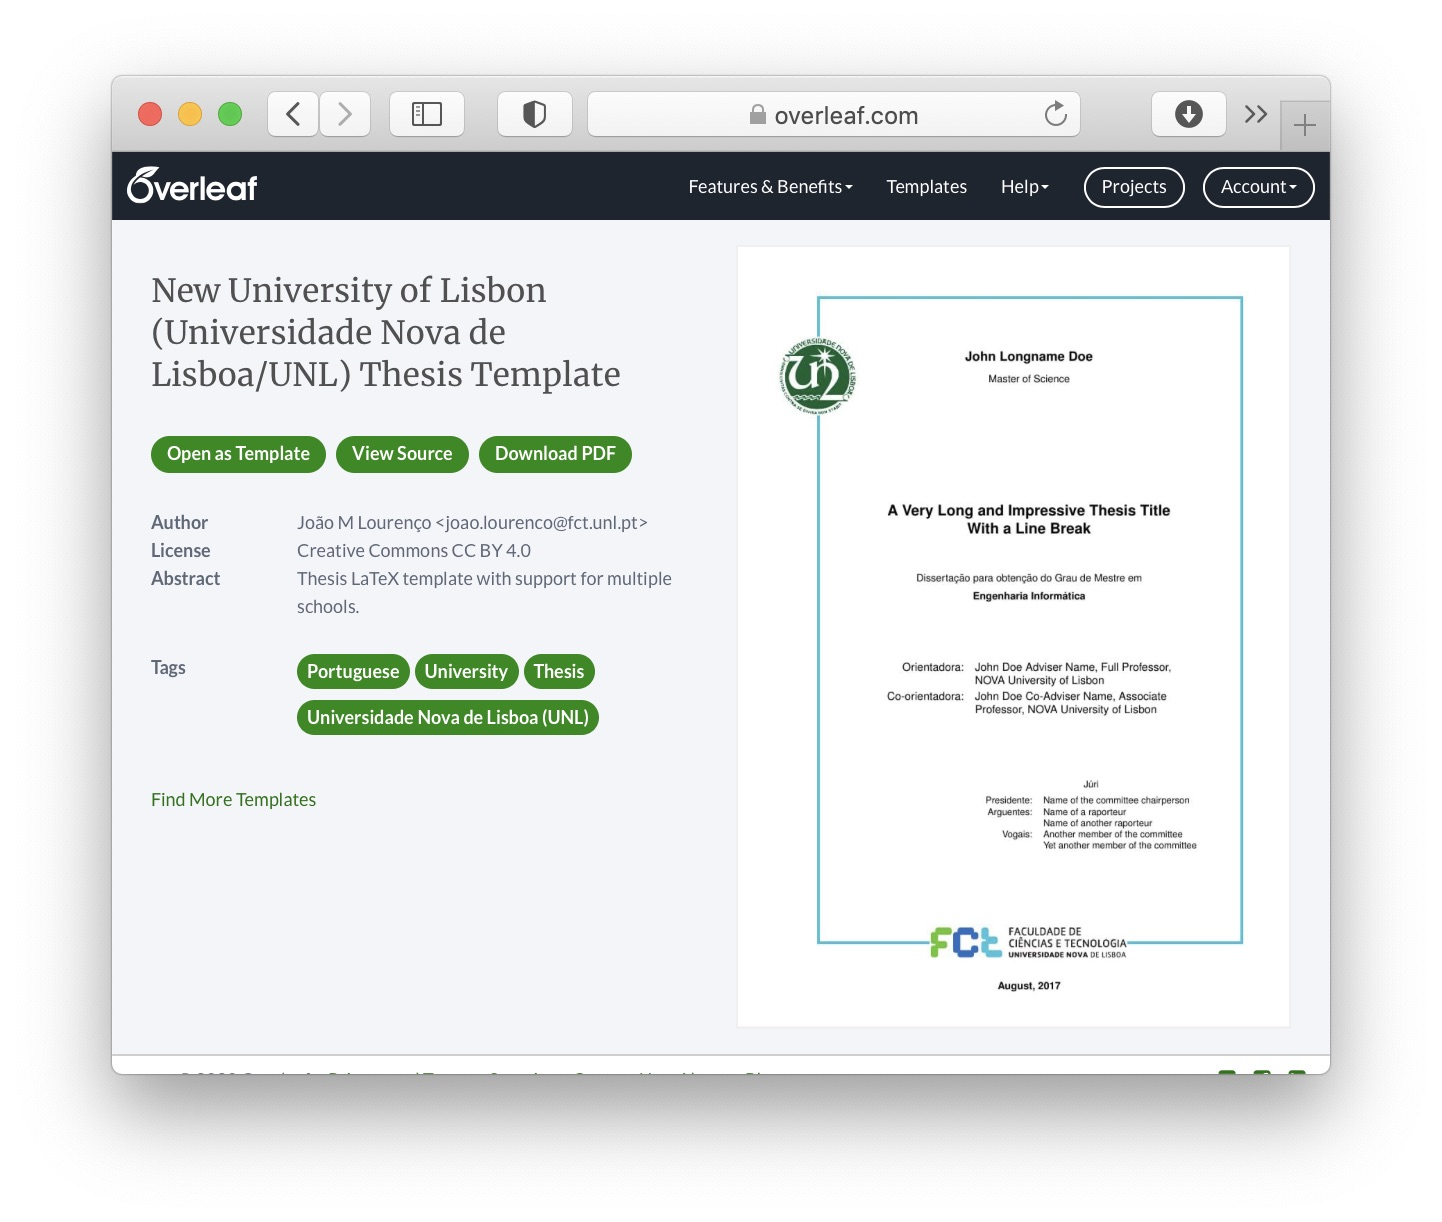
\includegraphics[width=\linewidth]{overleaf}%
\end{wrapfigure}

If you do not have an account in \href{https://www.overleaf.com?r=f5160636&rm=d&rs=b}{Overleaf}, you must \href{https://www.overleaf.com?r=f5160636&rm=d&rs=b}{create one first}.

Once you have an account, please access the \gls{novathesis} template in \href{https://www.overleaf.com/latex/templates/new-university-of-lisbon-universidade-nova-de-lisboa-slash-unl-thesis-template/fwbztcrptjmg}{Overleaf} and select the green button \emph{Open as Template}. 

\bgroup
  \itshape
  Please notice that the version currently available in Overleaf (v6.5.3) is slightly outdated. A new version will be submitted to Overleaf soon.  Until then, please:
  \begin{enumerate}
    \item Download the \href{https://github.com/joaomlourenco/novathesis/archive/master.zip}{latest version} from the GitHub repository as a Zip file.
    \item Login to your favorite LaTeX cloud service. I recommend \href{https://www.overleaf.com/?r=f5160636&rm=d&rs=b}{Overleaf} but there are alternatives (these instructions apply to Overleaf and you'll have to adapt for other providers).
    \item In the menu select: \texttt{New project} $\rightarrow$ \texttt{Upload project}.
    \item Upload the zip with all the “novathesis” files.
    \item Select “template.tex” as the main file.
    \item Let Overleaf compile the document.
  \end{enumerate}
\egroup

\subsection{Using a Local \LaTeX\ Installation}
\label{sub:using_local_latex}

\begin{wrapfigure}{r}{0.5\linewidth}
\vspace*{-15ex}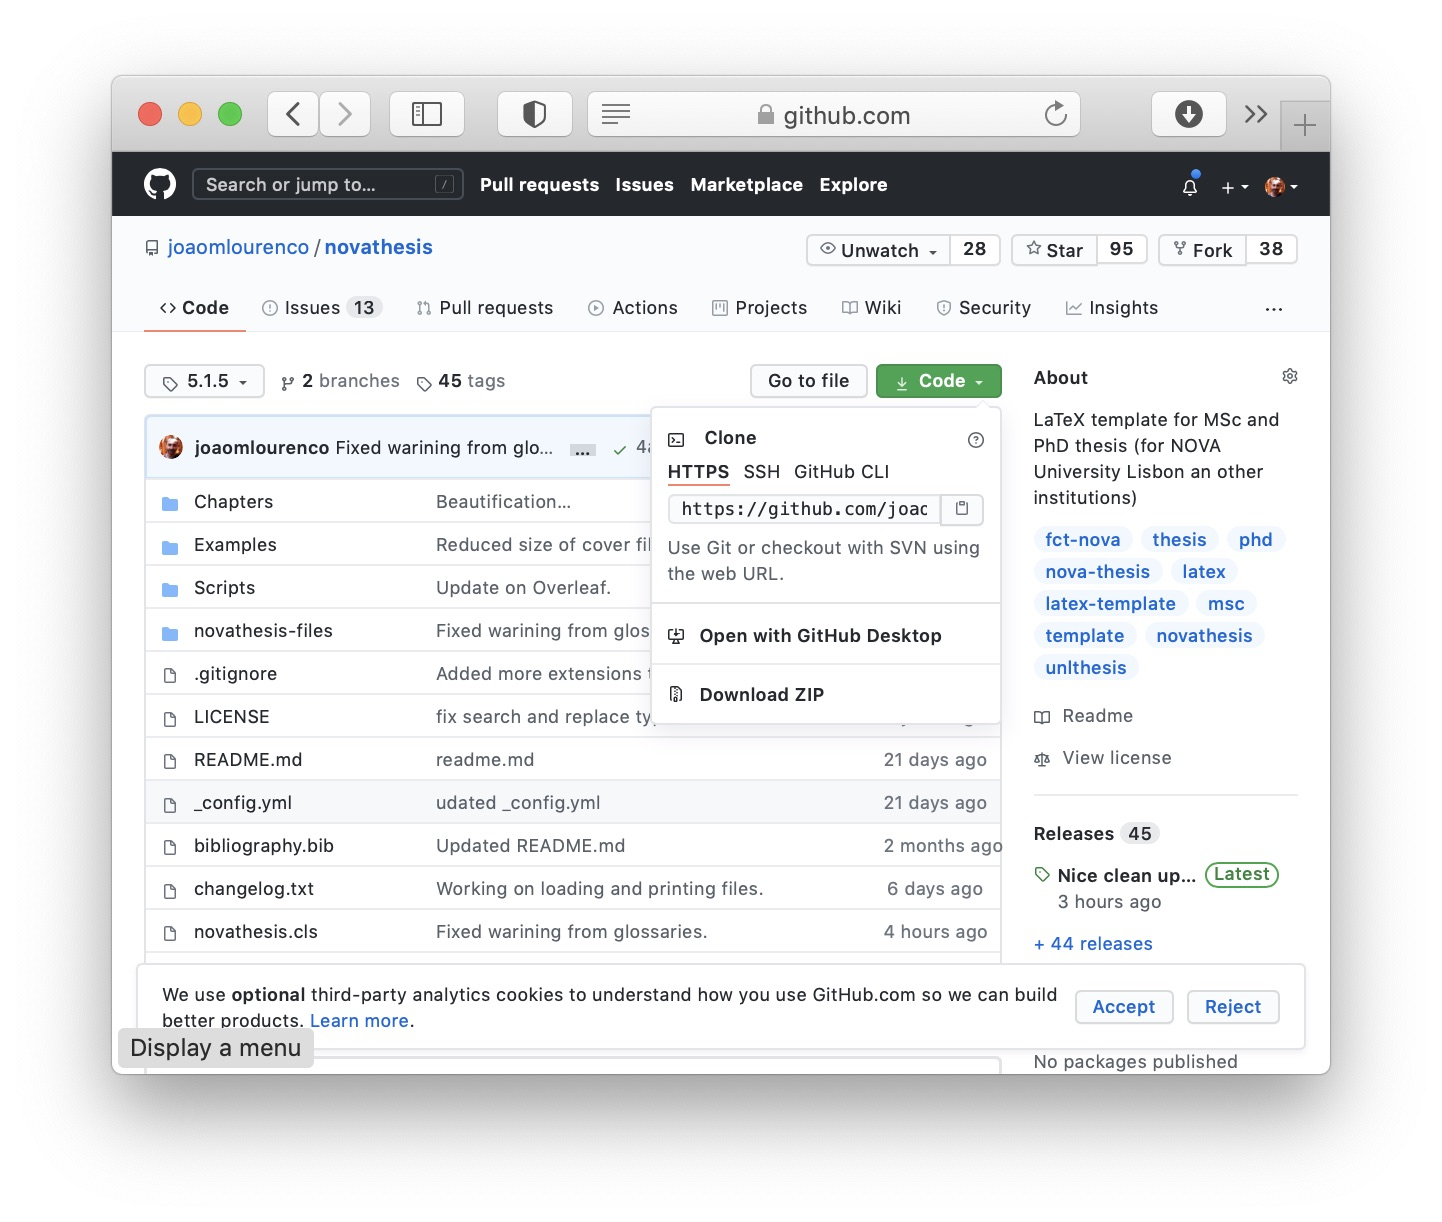
\includegraphics[width=\linewidth]{github}%
\end{wrapfigure}

Just access the \gls{novathesis} repository in \href{https://github.com/joaomlourenco/novathesis}{GitHub}, select the green button \emph{Code} and then \emph{download} (or \emph{clone}) the template.  You will always get the latest version of the template (currently v5.1.8).


\section{Getting Help}
\label{sec:getting_help}

Help is available in the forums listed below!

\begin{center}  
  \fbox{\parbox{0.95\textwidth}{\begin{center}\large\textbf{Please do not attempt to contact me directly (email, Messenger, etc)…\\I WILL NOT REPLY!}\end{center}}}
\end{center}
 
\subsection{Google}
\label{sub:group_google}

Remember, when looking for hints or help, \emph{\href{google.com}{Google} is your best friend}!   And if you prefix your Google query with “\emph{LaTeX}”, your fist link will most probably direct you to \texttt{tex.stackexchange.com}.

\subsection{Group Support}
\label{sub:group_support}

To get directed help on the \gls{novathesis} please join:
\begin{itemize}
  \item the \href{https://www.facebook.com/groups/novathesis}{NOVAtheis Facebook group}, or
  \item the \href{https://github.com/joaomlourenco/novathesis/discussions}{GitHub Discussions page}.
\end{itemize}

There were huge changes from version 4.x.y to version 6.a.b so, please, \textbf{always} state the version number you are using when asking for help.

\subsection{Reporting Problems}
\label{sub:reporting_problems}

If you just need some help, see above \Autoref{sub:group_google} and \Autoref{sub:group_support}.

If you believe \emph{you found a bug} or if \emph{you need some improvement} in the template, please \href{https://github.com/joaomlourenco/novathesis/issues}{fill an issue} in the \gls{novathesis} \href{https://github.com/joaomlourenco/novathesis/issues}{project page in GitHub}.


\section{Donors}
\label{sec:donations}

The \href{https://github.com/joaomlourenco/novathesis/wiki#donators}{list of \emph{Donnors}} is available in the \gls{novathesis} Project page.


\section{Disclaimer}
\label{sec:disclaimer}

Although the \gls{novathesis} template is endorsed by the FCT-NOVA (even \href{https://www.fct.unl.pt/estudante/informacao-academica}{linked from its web site}), this not an official template.
%
This template exists to make your life easier and we do our best to make it compliant to the supported Schools' regulations, but in the end of the line you and only you are accountable for both the look and the contents of the document you submit as your thesis/dissertation.

